\clearpage
\section{键合图优化}

\subsection{键合图因果划添加步骤}

\begin{itemize}
	\item 势源 $S_e$ 为势流出,所以因果划标在半箭头的外端;
	\item 势源 $S_f$ 为流流出,所以因果划标在半箭头的内端;
	\item 储能元件 $C I$ 先确定为积分因果关系,则 $C$ 元件的因果划标在半箭头的外端, $I$ 元件的因果划标在半箭头的内端;
	\item 0结为共势结,只能有一个流流出;
	\item 1结为共流结,只能有一个势流出;
	\item 结合 GY 和 TF 回转器和变换器的指定标法进行标注;
	\item 按照上面的原则对MPW和MDM的键合图标注因果划:
\end{itemize}

\subsection{MPW 系统键合图修改和简化}

\subsubsection{系统初步添加因果划}

据因果划的添加原则,对键合图初步添加因果划,如下图所示:
%%%%%%%%%%%%%%%%%
\begin{figure}[H]
	\centering
	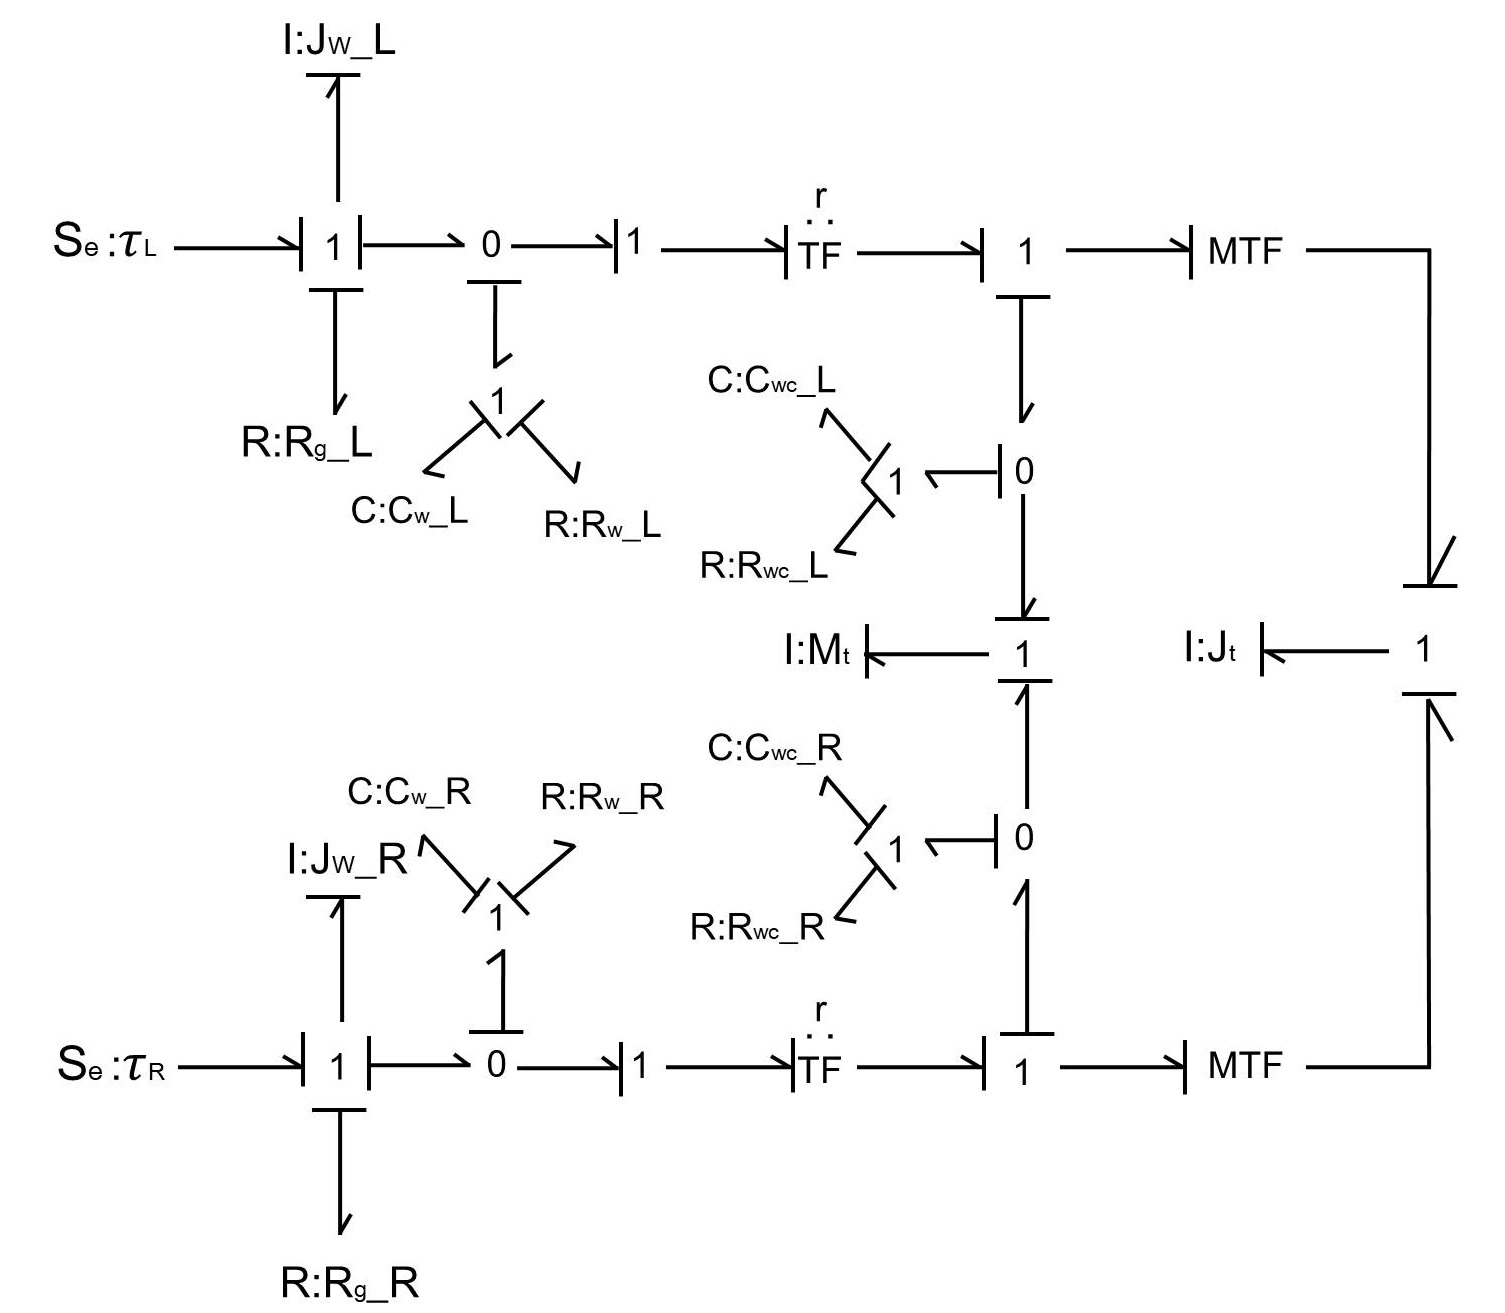
\includegraphics[width=0.6\textwidth]{fig/bond/MPW1.png}
	\caption{MPW系统因果划视图 }\label{fig:MPW1}
\end{figure}
%%%%%%%%%%%%%%%%%

\subsubsection{MPW系统键合图优化}

对于报告一中MPW模块的键合图,我们在此做了部分修改和优化,修改和优化后的部分如下图中红色方框中所示:
%%%%%%%%%%%%%%%%%
\begin{figure}[H]
	\centering
	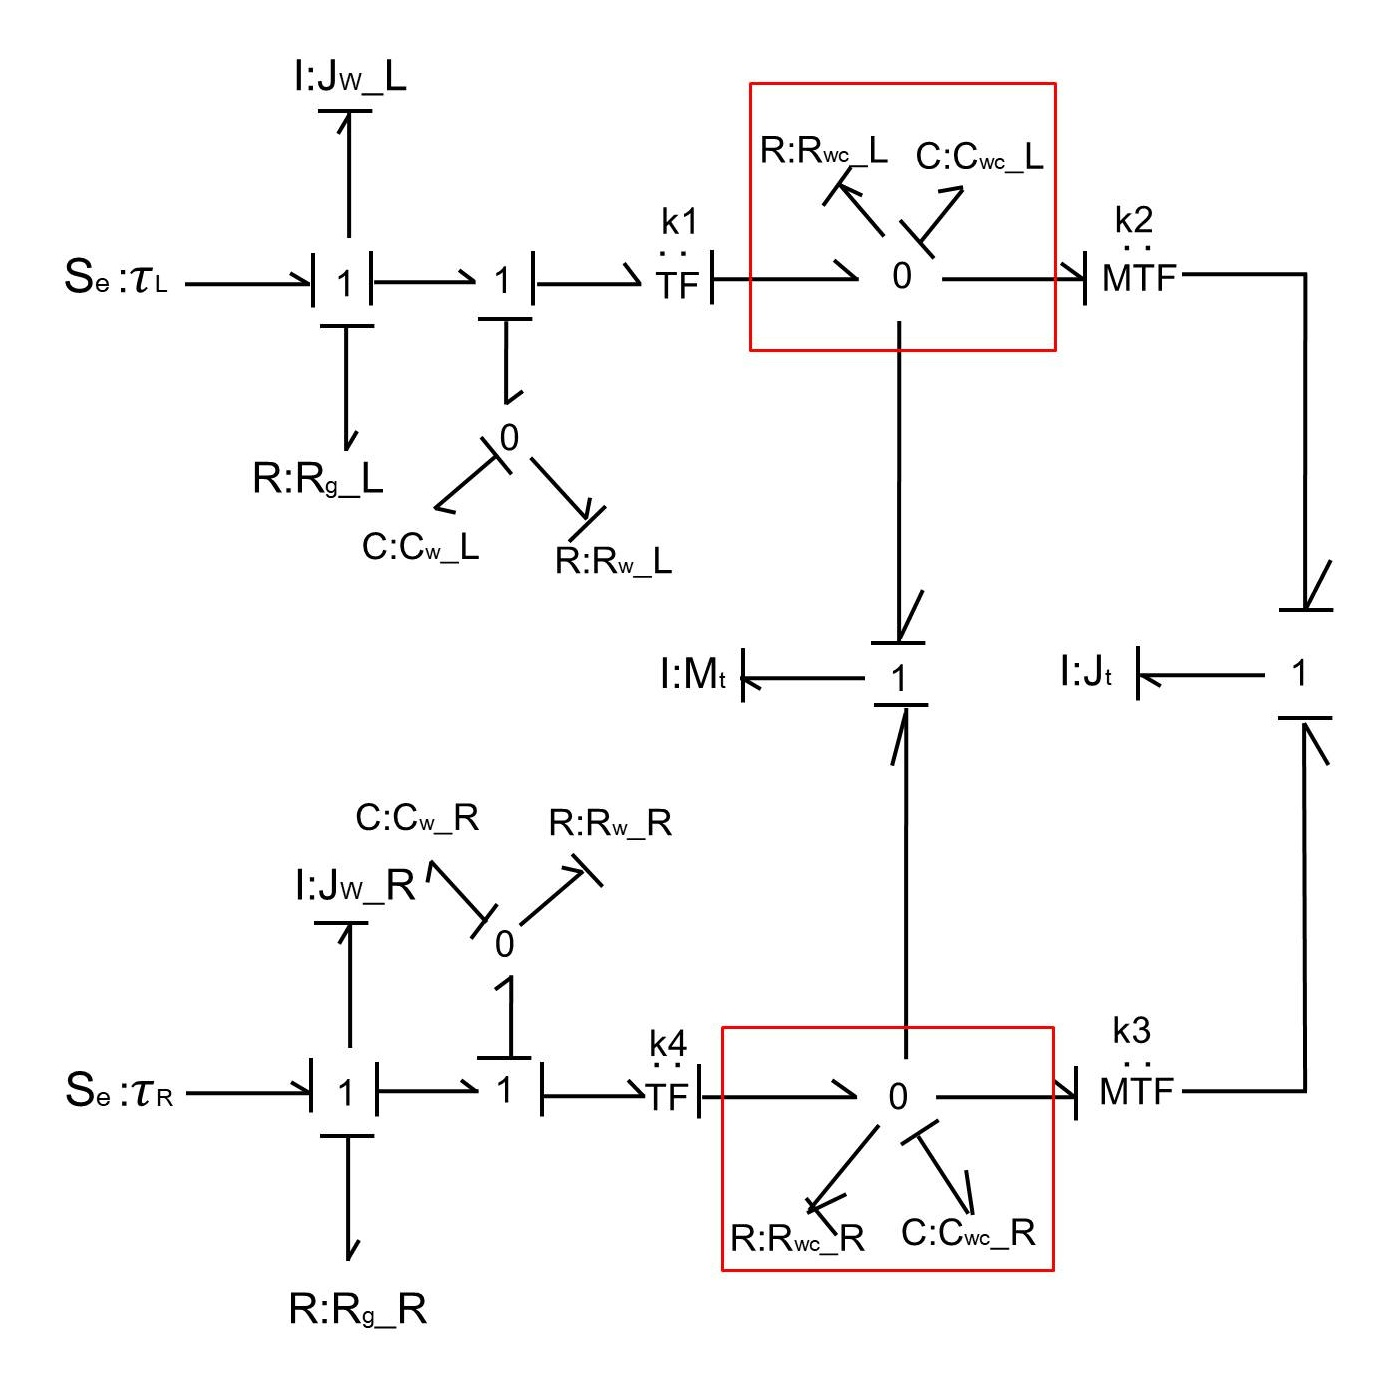
\includegraphics[width=0.6\textwidth]{fig/bond/MPW2.png}
	\caption{MPW系统优化键合图}\label{fig:MPW2}
\end{figure}
%%%%%%%%%%%%%%%%%

\subsection{MDM 系统键合图修改和简化}

\subsubsection{左轮电机模块简化与因果划添加}

根据因果划的添加原则,对电机模块的键合图初步添加因果划,如下图所示:
%%%%%%%%%%%%%%%%%
\begin{figure}[H]
	\centering
	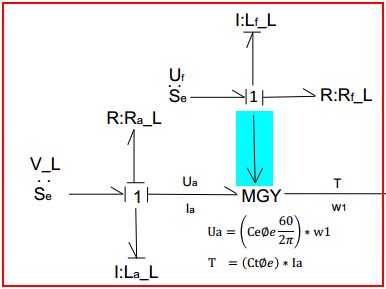
\includegraphics[width=0.5\textwidth]{fig/bond/MDM1.png}
	\caption{左轮电机模块因果划视图}\label{fig:bond_MDM1}
\end{figure}
%%%%%%%%%%%%%%%%%

对于他励直流电动机的驱动原理,电动机回路中电枢电压、电枢电流与电动机输出扭矩、输出角速度之间存在一个回转器的关系,如果励磁回路中的驱动磁场是变化的,则此回转器属于可变回转器MGY,励磁磁场直接影响的大小$ \Phi_e $,所以影响 $U_a=\left(C_e \Phi_e \frac{60}{2 \pi}\right) * w$ 和 $T=(C_t \Phi_e) * I_a$ 中的比例关系,属于可变回转器,为了简化实验,我们决定采用的是恒励磁磁场的模式,即励磁回路中的磁场恒定,所以此回转器属于定值回转器,并设定其系数为$ K_1 $,简化后的电机模块键合图如下图所示:
%%%%%%%%%%%%%%%%%
\begin{figure}[H]
	\centering
	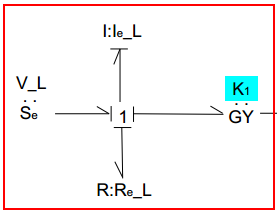
\includegraphics[width=0.5\textwidth]{fig/bond/MDM2.png}
	\caption{左轮电机模块简化键合图}\label{fig:bond_MDM2}
\end{figure}
%%%%%%%%%%%%%%%%%

同理可得右轮电机模块简化键合图。

\subsubsection{机械部分键合图简化与因果划添加}

根据因果划的添加原则,对MDM机械部分的键合图初步添加因果划,如下图所示:
%%%%%%%%%%%%%%%%%
\begin{figure}[H]
	\centering
	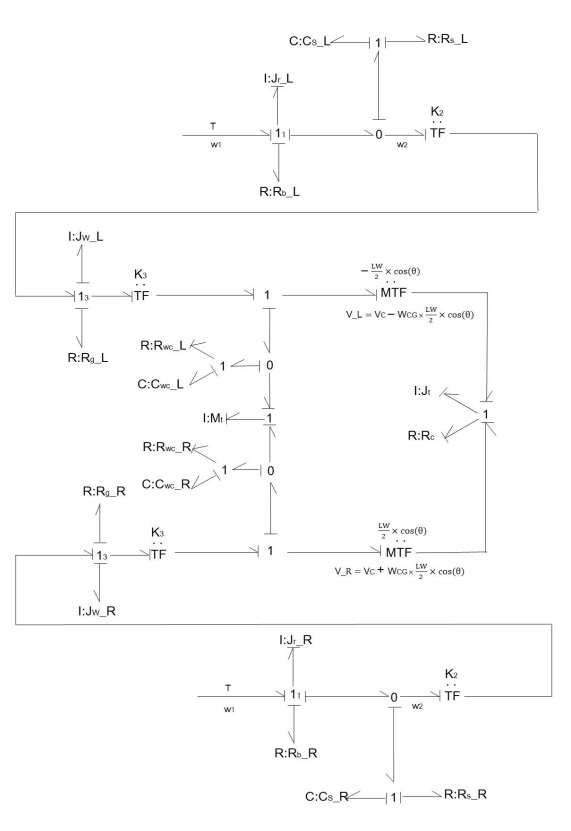
\includegraphics[width=0.55\textwidth]{fig/bond/MDM3.png}
	\caption{MDM机械部分因果划视图}\label{fig:bond_MDM3}
\end{figure}
%%%%%%%%%%%%%%%%%

为了方便仿真,我们对图进行来部分优化和修改优化,如下所示:
%%%%%%%%%%%%%%%%%
\begin{figure}[H]
	\centering
	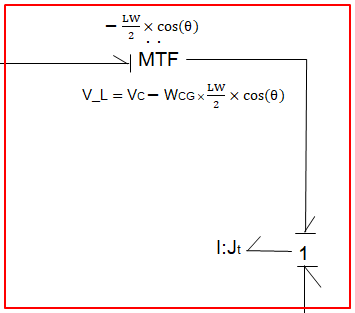
\includegraphics[width=0.5\textwidth]{fig/bond/MDM4.png}
	\caption{左轮变换器键合图}\label{fig:bond_MDM4}
\end{figure}
%%%%%%%%%%%%%%%%%

根据物理模型,左轮的线速度、整体模型的质心线速度、整体模型的质心角速度之间存在如下关系式:$v_L=v_C-w_{CG} \cdot \frac{L_w \cos(\theta)}{2}$ ,整体模型水平偏角 $ \theta $ 是变化的,所以此处存在一个可变变换器,为了方便仿真,我们决定采用寻找左右轮线速度瞬心的方法来确定变换器的系数,这种方法更加简便,这在后面章节中详细介绍,所以此处我们可以把变换器简化为下图所示,其中系数 $K_4$ 是变量:
%%%%%%%%%%%%%%%%%
\begin{figure}[H]
	\centering
	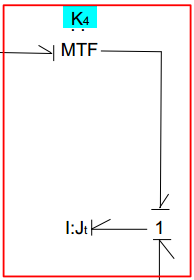
\includegraphics[width=0.35\textwidth]{fig/bond/MDM5.png}
	\caption{左轮变换器优化键合图}\label{fig:bond_MDM5}
\end{figure}
%%%%%%%%%%%%%%%%%

为了方便状态空间方程的建立,我们对报告一中的键合图两处进行了修改,修改后的键合图如下图所示,红色方框中为修改优化后的结果:
%%%%%%%%%%%%%%%%%
\begin{figure}[H]
	\centering
	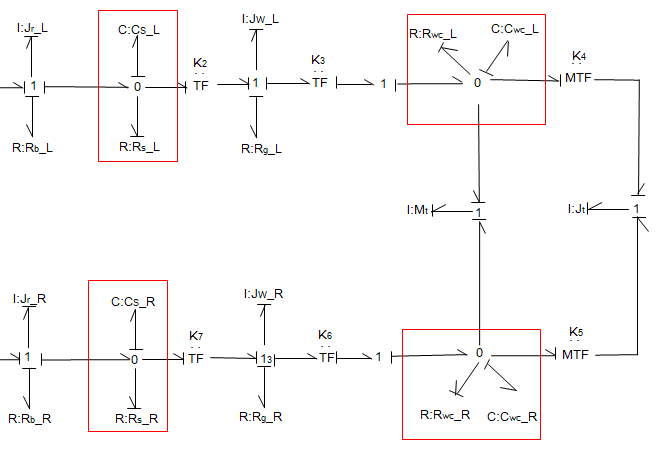
\includegraphics[width=0.8\textwidth]{fig/bond/MDM6.png}
	\caption{左轮变换器优化键合图}\label{fig:bond_MDM6}
\end{figure}
%%%%%%%%%%%%%%%%%

\subsubsection{MDM 模块的对接}

优化后的 MDM 总体键合图如下所示:
%%%%%%%%%%%%%%%%%
\begin{figure}[H]
	\centering
	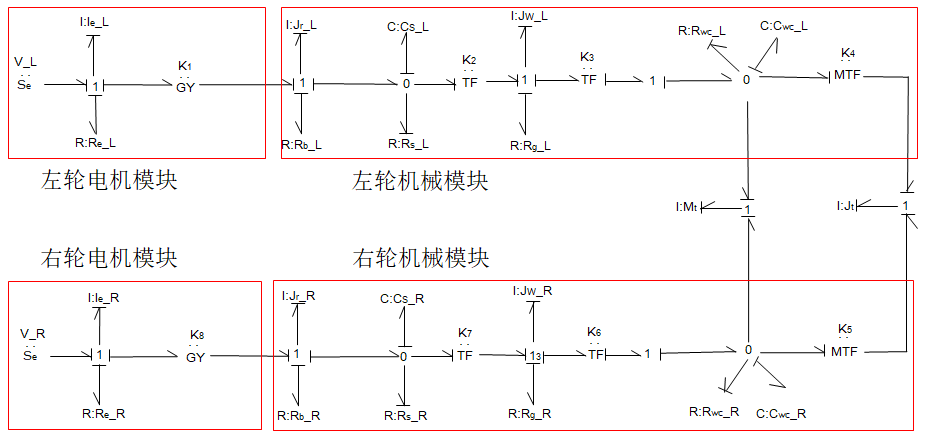
\includegraphics[width=0.8\textwidth]{fig/bond/MDM7.png}
	\caption{左轮变换器优化键合图}\label{fig:bond_MDM7}
\end{figure}
%%%%%%%%%%%%%%%%%
